\documentclass[12pt,longbibliography]{article}
\usepackage[utf8]{inputenc}
\usepackage[T1]{fontenc}
\usepackage[a4paper, margin=2.7cm]{geometry}

\usepackage{amsmath, amsthm, amsfonts, amssymb}
\newtheorem{thm}{Theorem}[section]
\newtheorem{cor}[thm]{Corollary}
\newtheorem{lem}[thm]{Lemma}
\newtheorem{prop}[thm]{Proposition}
\theoremstyle{definition}
\newtheorem{defn}[thm]{Definition}
\theoremstyle{remark}
\newtheorem{rem}[thm]{Remark}

\usepackage{mathrsfs} 
\usepackage[colorlinks=true,linkcolor=blue,citecolor=blue,urlcolor=blue,breaklinks]{hyperref}

\usepackage{bbm} 

\usepackage{hyperref}
\usepackage{graphicx}
\graphicspath{ {Imatges portada/} }

\title{Big Query}
\author{Anna Salazar}

\renewcommand{\contentsname}{Índex}
\renewcommand{\figurename}{Figura}
\renewcommand{\tablename}{Taula}

\begin{document}
\begin{titlepage}
\maketitle

\vspace{140mm}

\par
\raisebox{-.5\height}{
\includegraphics[width=6cm]{fme}}%
\hfill
\raisebox{-.5\height}{
\includegraphics[width=6cm]{UB}}%
\par

\end{titlepage}

\tableofcontents

\pagebreak

\pagenumbering{arabic}

\section{Què és BigQuery?}

BigQuery és un motor d’anàlisi de macrodades (Big Data) que permet executar consultes SQL al núvol sobre les dades emmagatzemades en aquest, sense importar el volum de les dades ni el tipus de consultes que es volen fer. El motor de consulta és capaç de treballar sobre terabytes de dades en qüestió de segons, i sobre petabytes en pocs minuts. Avui en dia, les empreses estan adoptant cada cop més la presa de decisions basades en dades i fomentant una cultura oberta en la qual les dades no estan aïllades dins dels departaments. BigQuery, en proporcionar els mitjans tecnològics per a promoure un canvi cultural cap a l’agilitat i l’obertura, realitza un paper molt important en l’augment del ritme de la innovació.

\vspace{2mm}

Treballar amb dades a BigQuery implica 3 aspectes principals: l’emmagatzemament, la incorporació de les dades i la consulta d’aquestes, Google s’encarrega de tota la resta. Com BigQuery és un servei totalment gestionat, no és necessari configurar ni instal·lar res en el nostre ordinador i, pel mateix motiu, no necessitem un administrador de la base de dades. Simplement, podem entrar en el nostre projecte de Google Cloud des del nostre navegador i començar a analitzar.

\vspace{2mm}

Pel que fa a l’emmagatzemament, les dades es guarden en una taula estructurada, la qual cosa significa que es pot utilitzar l’SQL estàndard per a facilitar la consulta i l’anàlisi de dades. BigQuery és perfecta pel Big Data perquè gestiona tot aquest emmagatzemament i està proveïda d’operacions d’escalabilitat que funcionen de forma automàtica sense que l’usuari s’hagi d’involucrar,  per la qual cosa mai haurem de preocupar-nos per la grandària de les dades amb els quals treballem. Part de la consideració de disseny darrere de BigQuery és animar als usuaris a centrar-se en els coneixements en lloc de la infraestructura. Quan s’introdueixen les dades a BigQuery no és necessari pensar en els diferents tipus d’emmagatzemament, ni en els seus avantatges pel que fa a velocitat i cost; l’emmagatzemament està totalment gestionat.

\vspace{2mm}
\noindent
Per a més informació sobre BigQuery, es pot consultar la pàgina de \href{https://cloud.google.com/bigquery/docs/introduction}{Google Cloud}.

\subsection{Per què hauríem d'utilitzar BigQuery en lloc d'altres eines?}

Una de les característiques més rellevants que presenta BigQuery és que es tracta d'una plataforma sense servidor, és a dir, que els servidors s'executen en segon pla, sense l'intervenció de l'usuari. A més, presenta una alta disponibilitat, la qual cosa es tradueix en que no cal preocupar-se per la caiguda dels servidors, ja que el servei s'encarrega d'això. Per últim, BigQuery també té propietats d'escalabilitat automàtica que fan possible gestionar fins a petabytes de dades. Aquestes característiques no estan disponibles a la majoria de plataformes d'emmagatzament de dades tradicionals, cosa que fa destacar BigQuery entre moltes.

\vspace{2mm}

Com en molts altres magatzems de dades, BigQuery és capaç de treballar amb moltes fonts de dades diferents. Pot extreure dades del seu propi sistema d'arxius, de Google Cloud Storage i de moltes fonts més. Després de fer-ho, es poden consultar aquestes dades utilitzant SQL estàndard o SQL heretat, el rendiment en qualsevol cas és excel·lent. Els resultats de les consultes solen emmagatzemar-se en la memòria cau durant 24 hores, de manera que les següents execucions d'aquesta consulta només hauran d'obtenir les dades de la cau en lloc de fer-ho del disc. 


\pagebreak

\section{Creació i treball amb conjunts de dades i taules}

\subsection{Configuració de la Plataforma de Google Cloud (GCP)}

\graphicspath{ {BigQuery/Imatges tutorial/} }

Per utilitzar aquesta eina d’anàlisi només ens caldrà crear un compte a Google Cloud i treballar a la zona de proves que ofereix Google per treballar de forma gratuïta.
Per fer servir la zona de proves (Sandbox) seguirem els passos següents: 

1. En primer lloc, ens dirigim a la interfície d’usuari de \href{https://console.cloud.google.com}{BigQuery.}. Des d'aquesta interfície es poden realitzar la majoria de les operacions.

2. Accedeix al teu compte de Google o crea un nou compte si encara no en tens cap. Si és el primer cop que inicies sessió a Google Cloud, hauràs de marcar el país i acceptar les condicions de servei.

3. Un cop dins, podem veure com és l'espai de treball SQL. Hi ha una secció de l'Explorador a l'esquerra que ens permet navegar en projectes, conjunts de dades i taules.Per tal de fer servir la zona de proves, haurem de crear un projecte.

\begin{center}
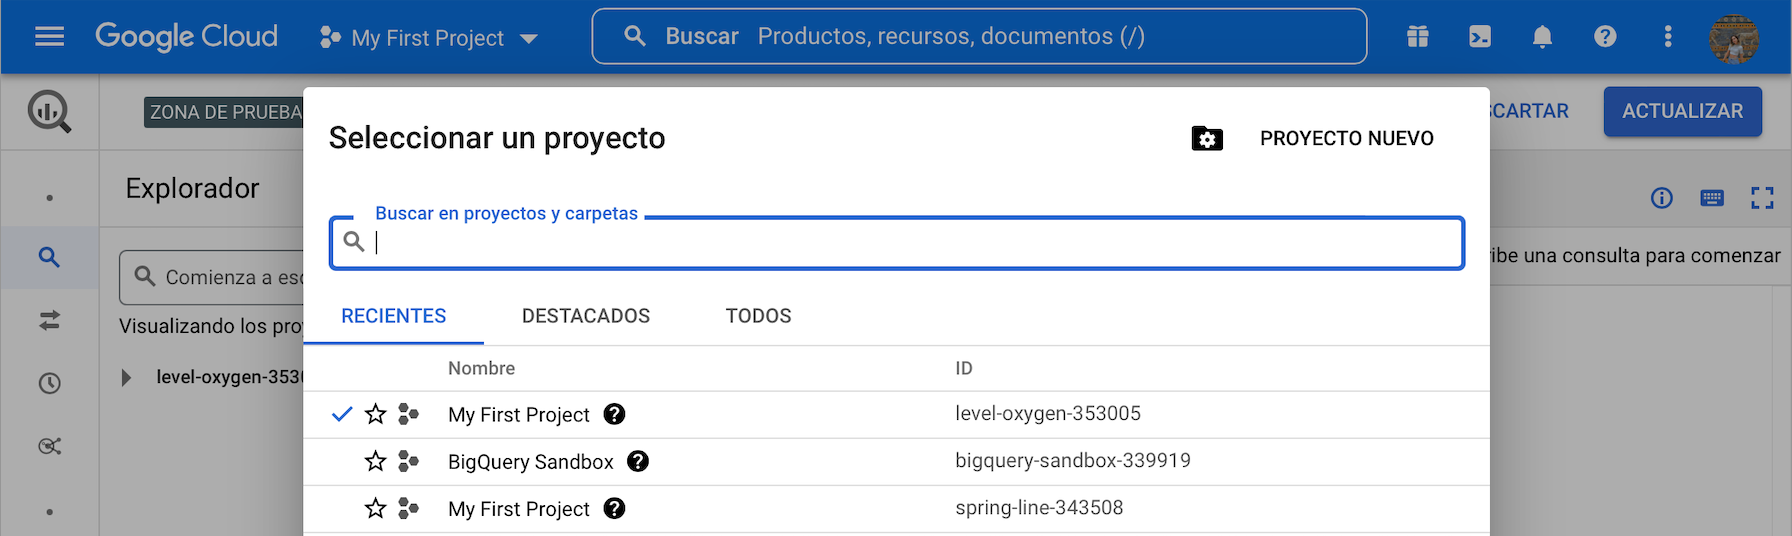
\includegraphics[width=7cm]{bq1}
\end{center}

Introdueix un nom al teu projecte i fes clic a Create. En el nostre cas, hem anomenat el projecte \textit{El meu projecte}, i treballarem sobre aquest per il·lustrar el funcionament de la plataforma.

\begin{center}
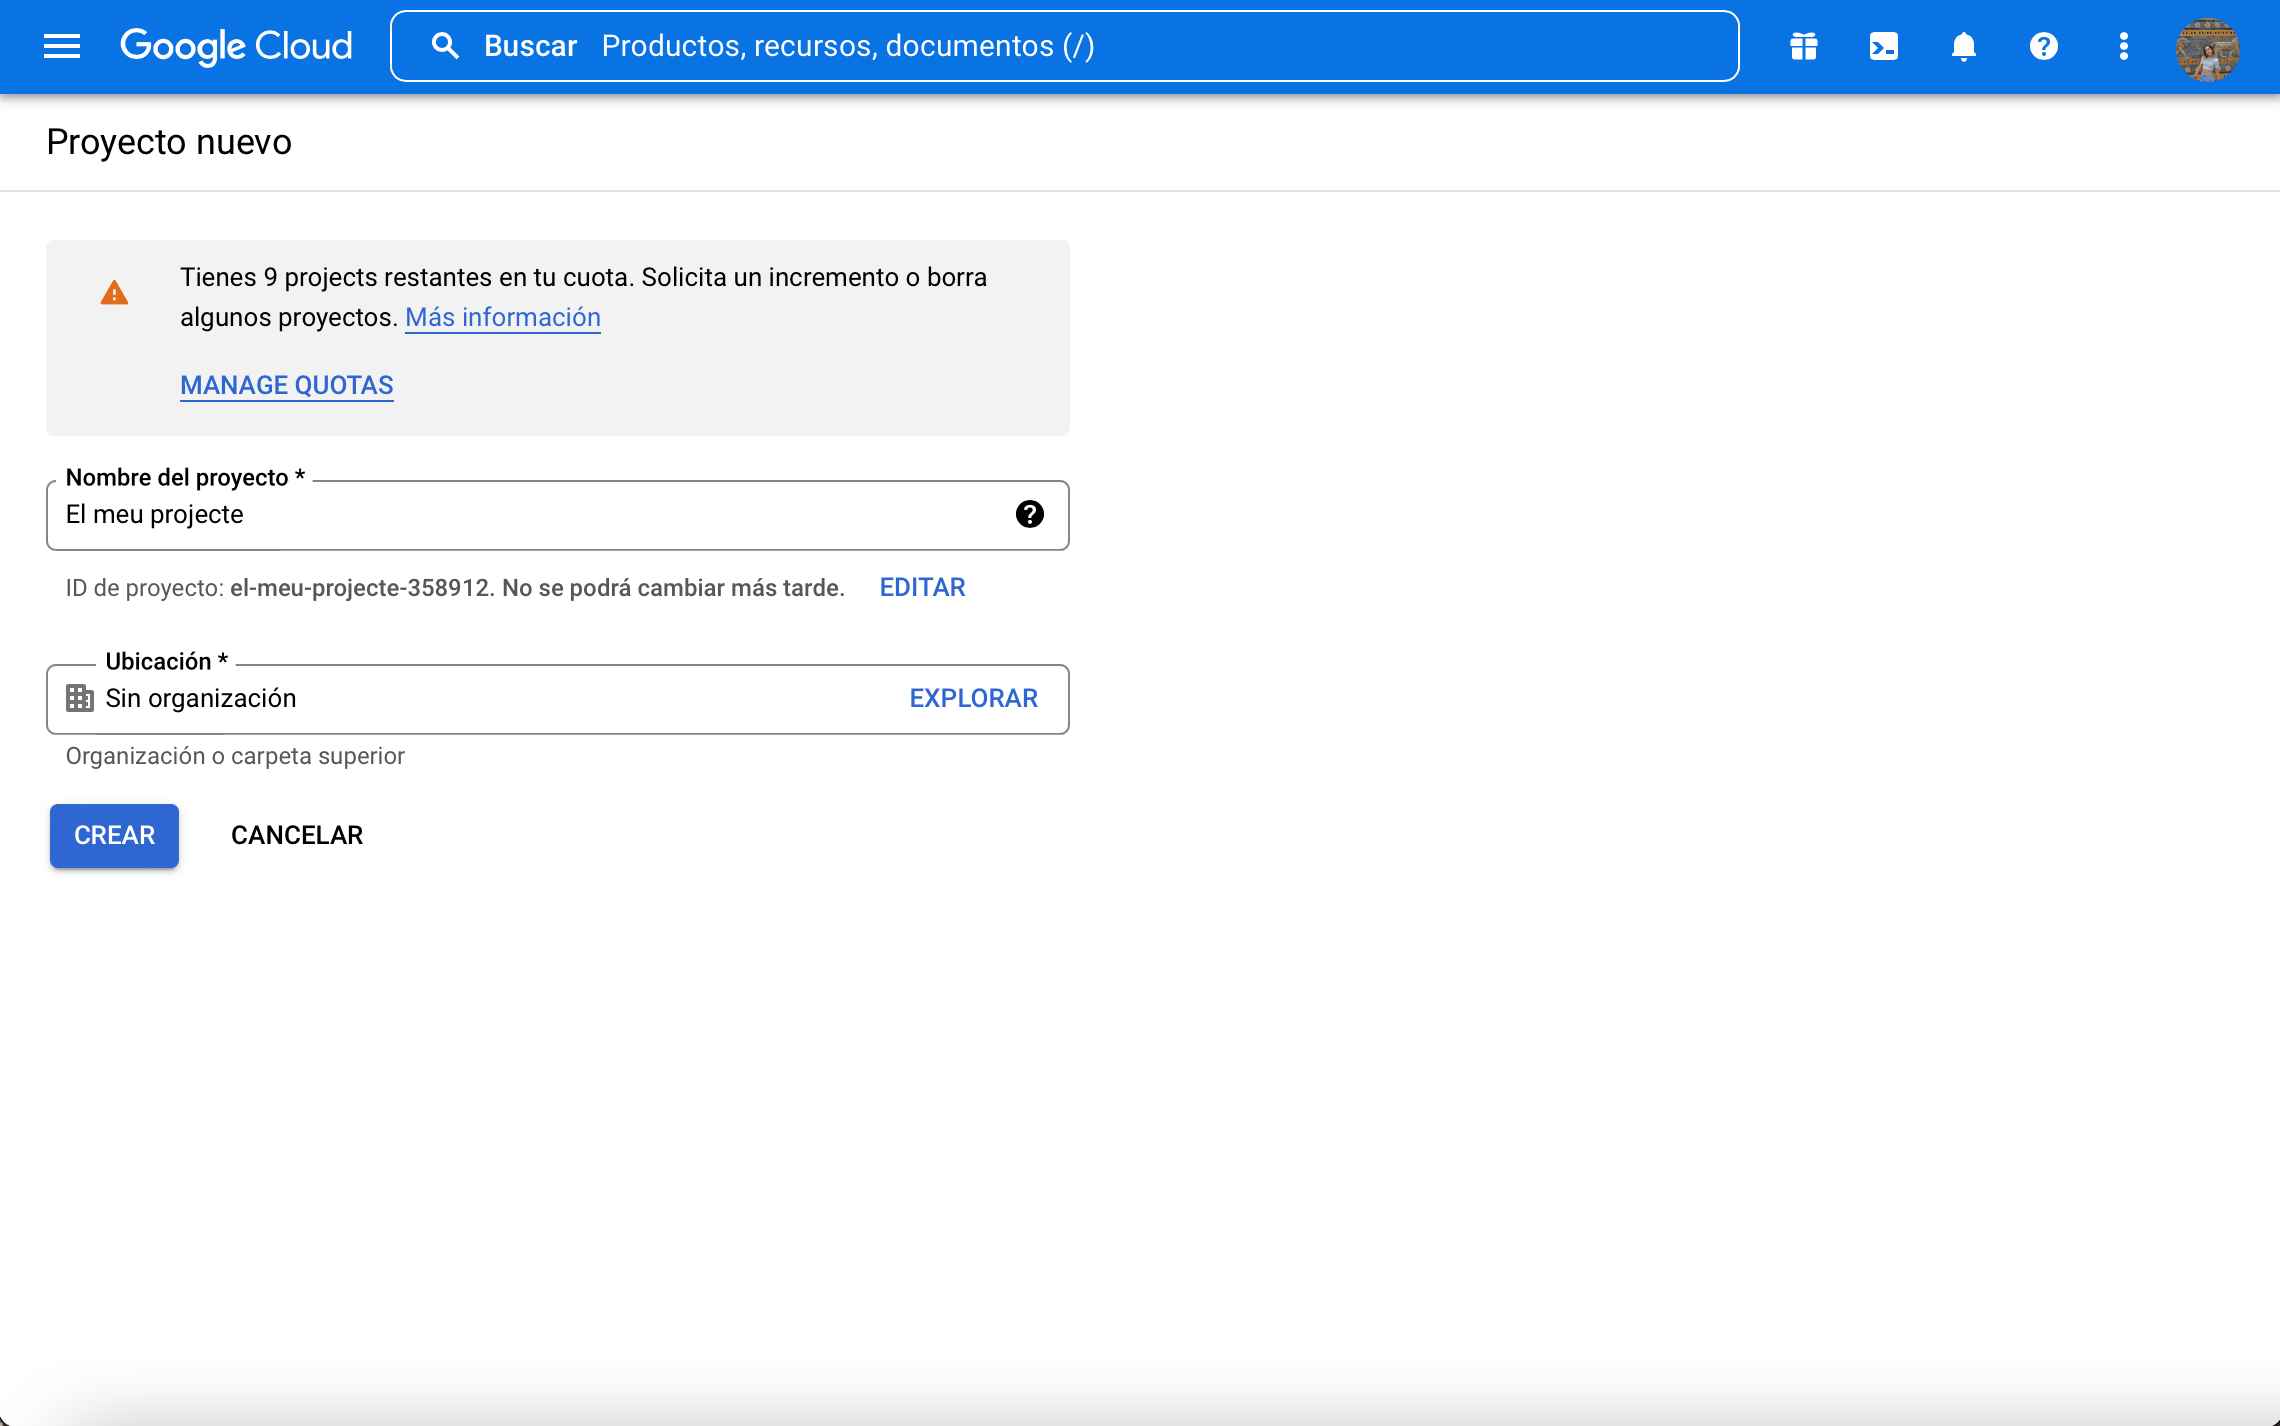
\includegraphics[width=7cm]{bq2}
\end{center}

4. Un cop creat el projecte, seràs redirigit a la interfície web de BigQuery.

5. Ara ja pots carregar o consultar dades en el teu projecte sense cap compte de
facturació adjunta.

\begin{center}
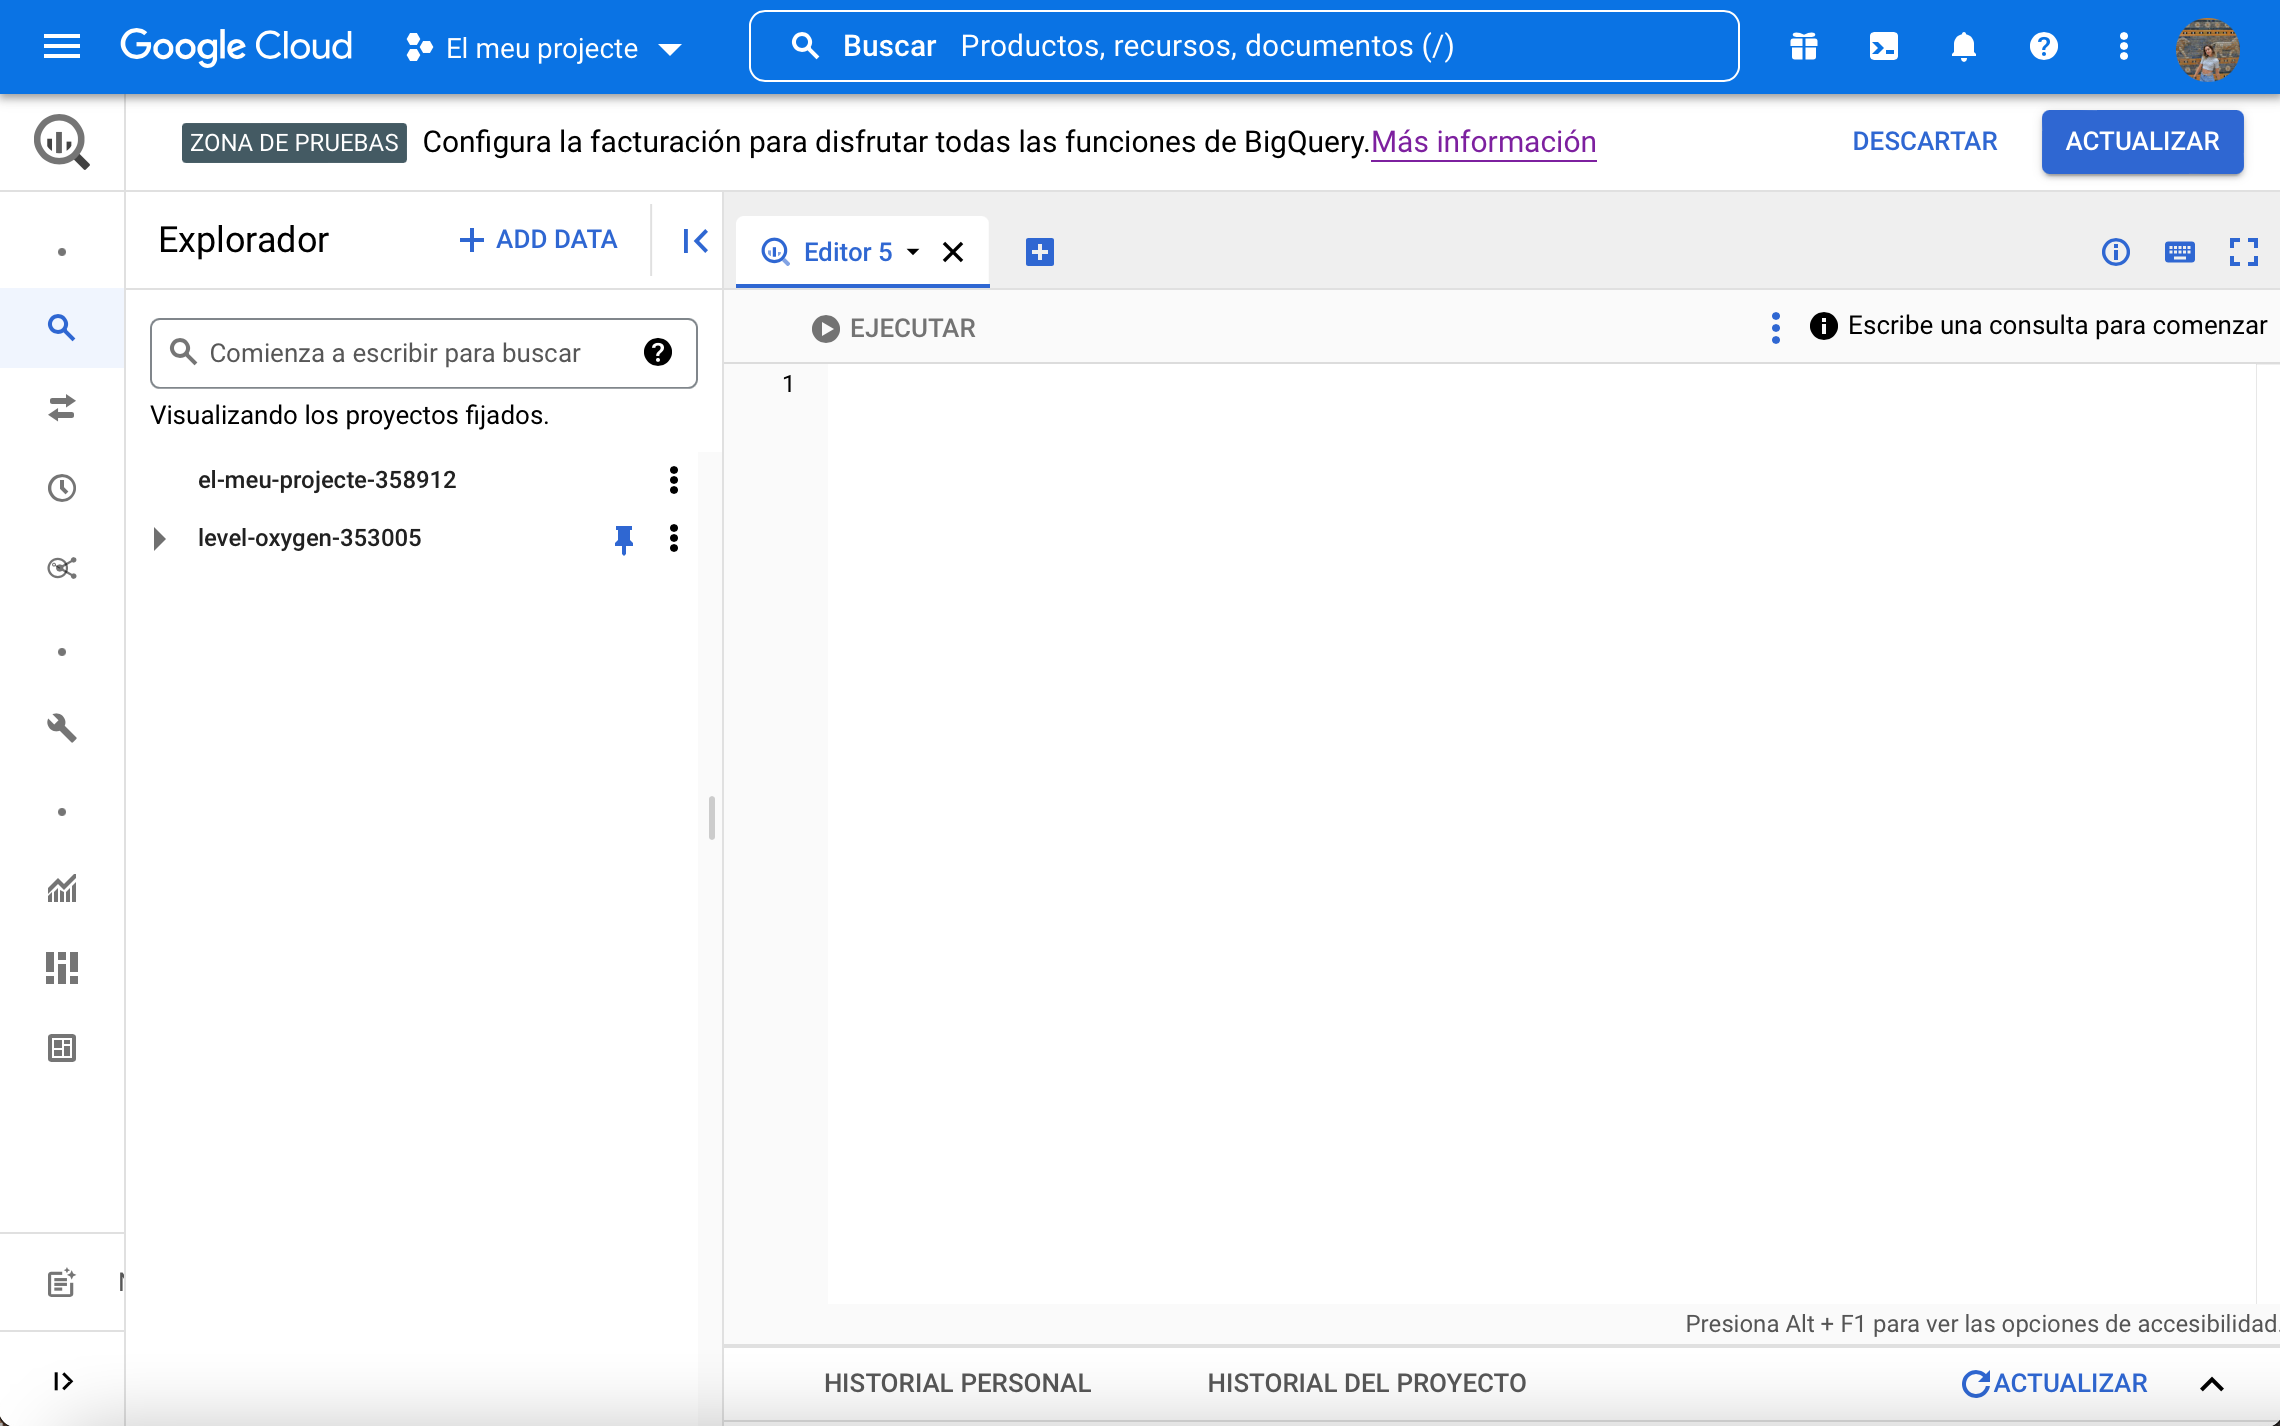
\includegraphics[width=7cm]{bq3}
\end{center}

\subsection{Creació d'un conjunt de dades}

\begin{center}
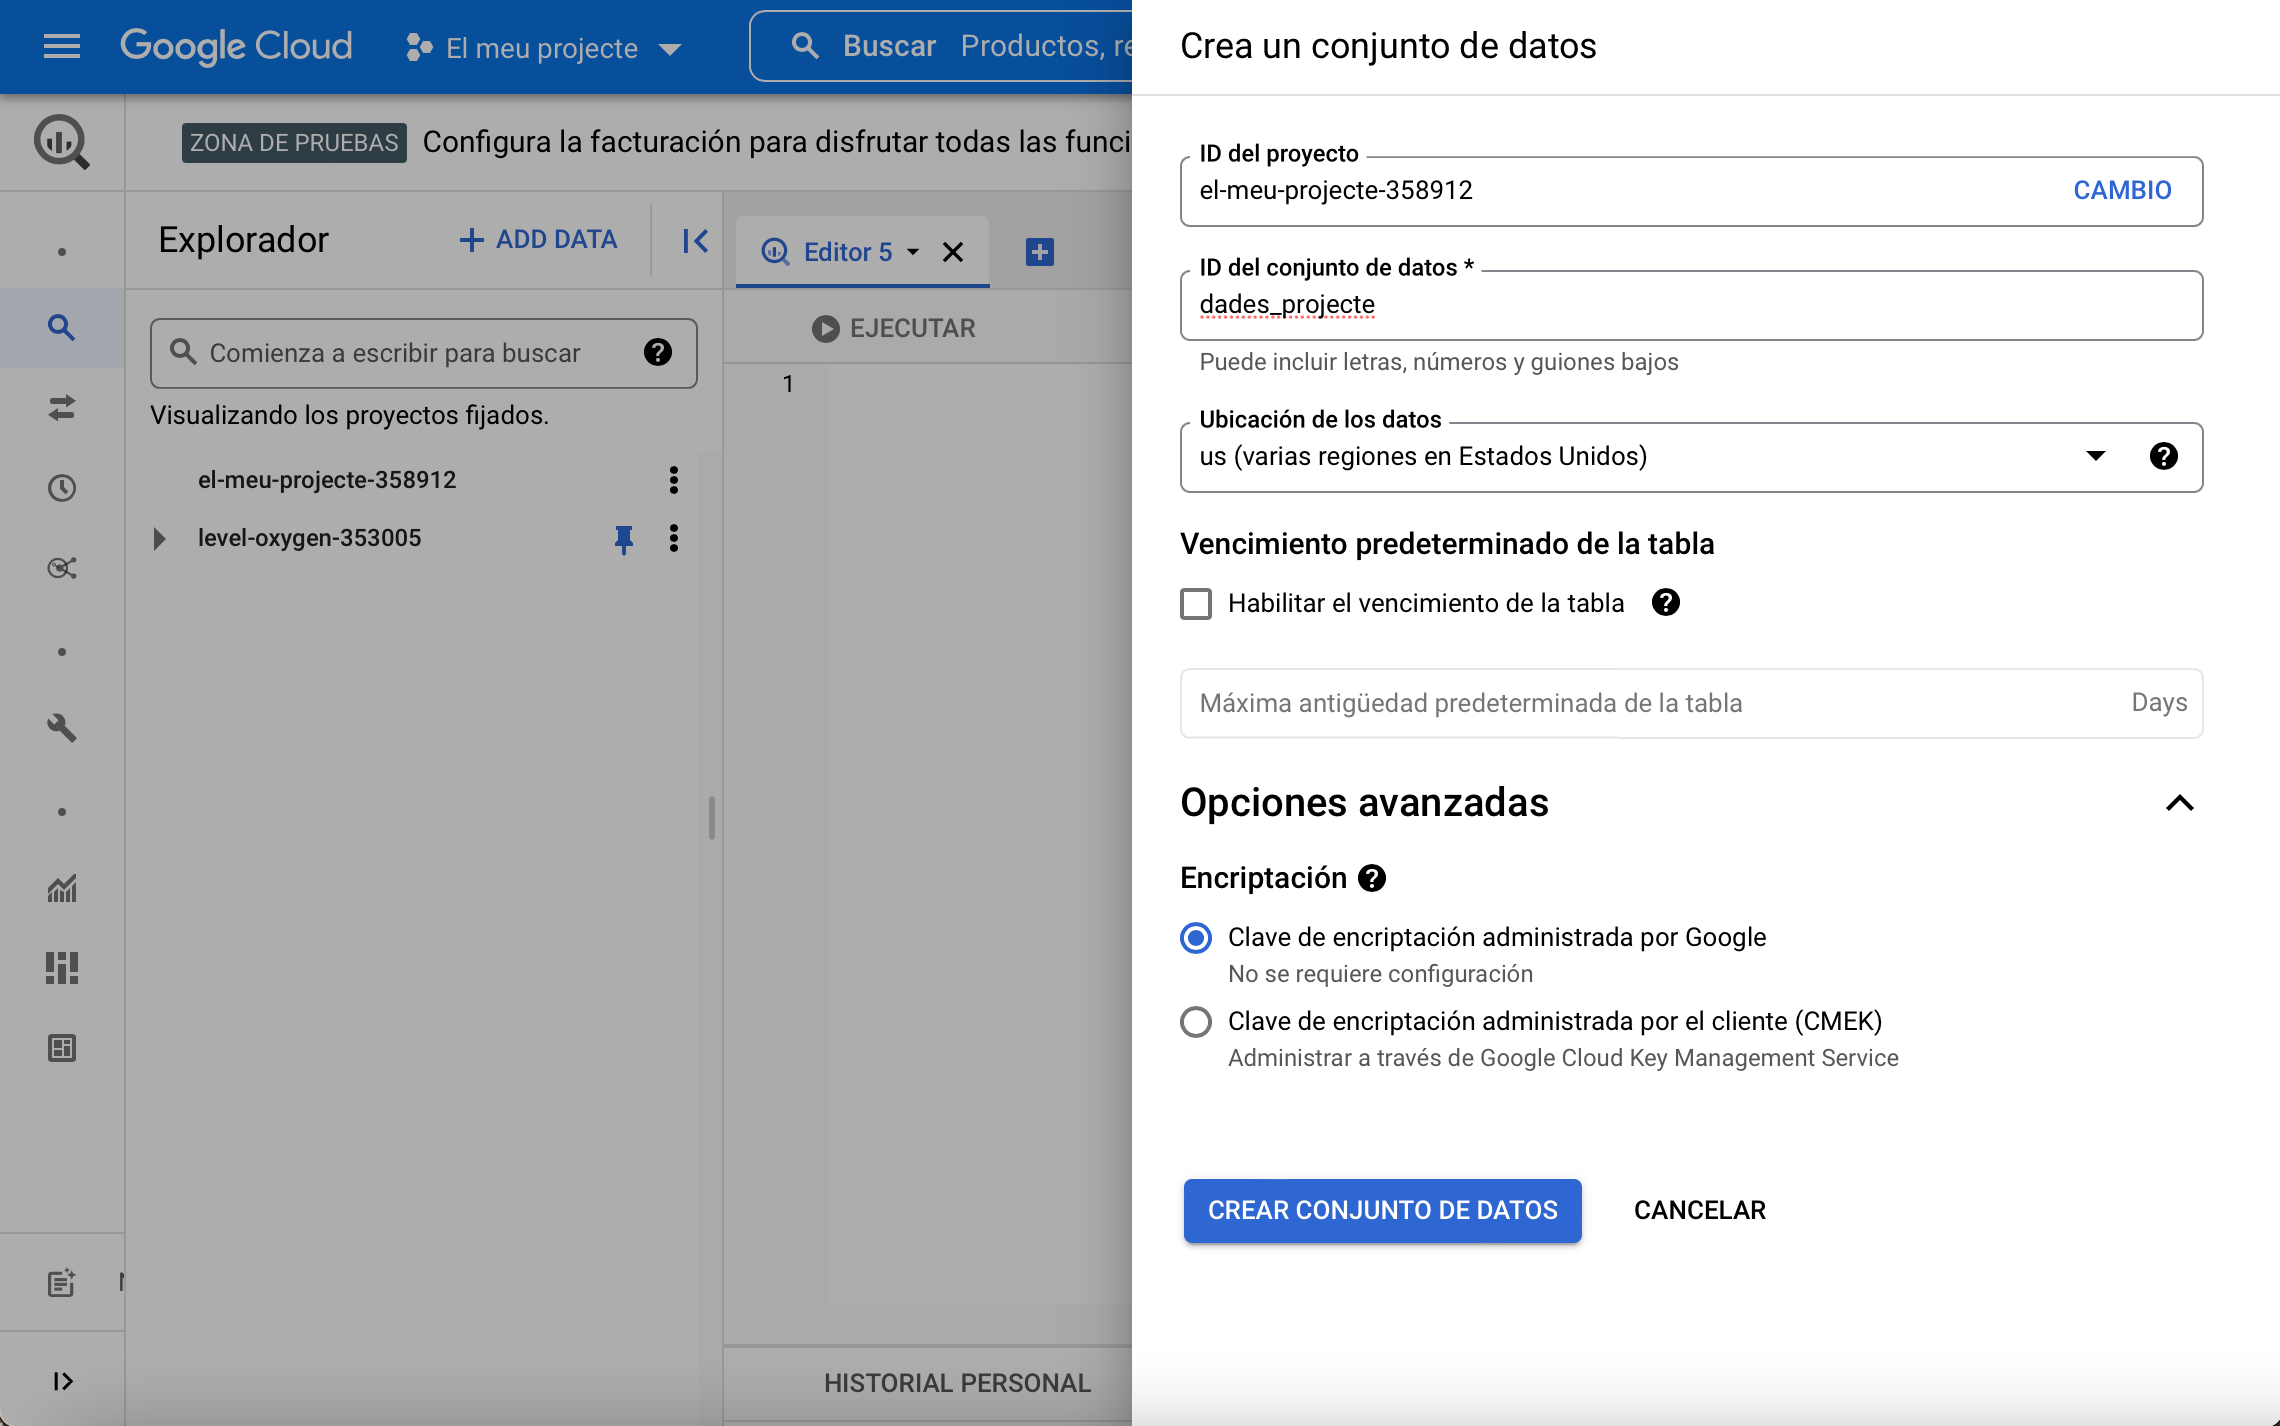
\includegraphics[width=7cm]{bq4}
\end{center}

\begin{center}
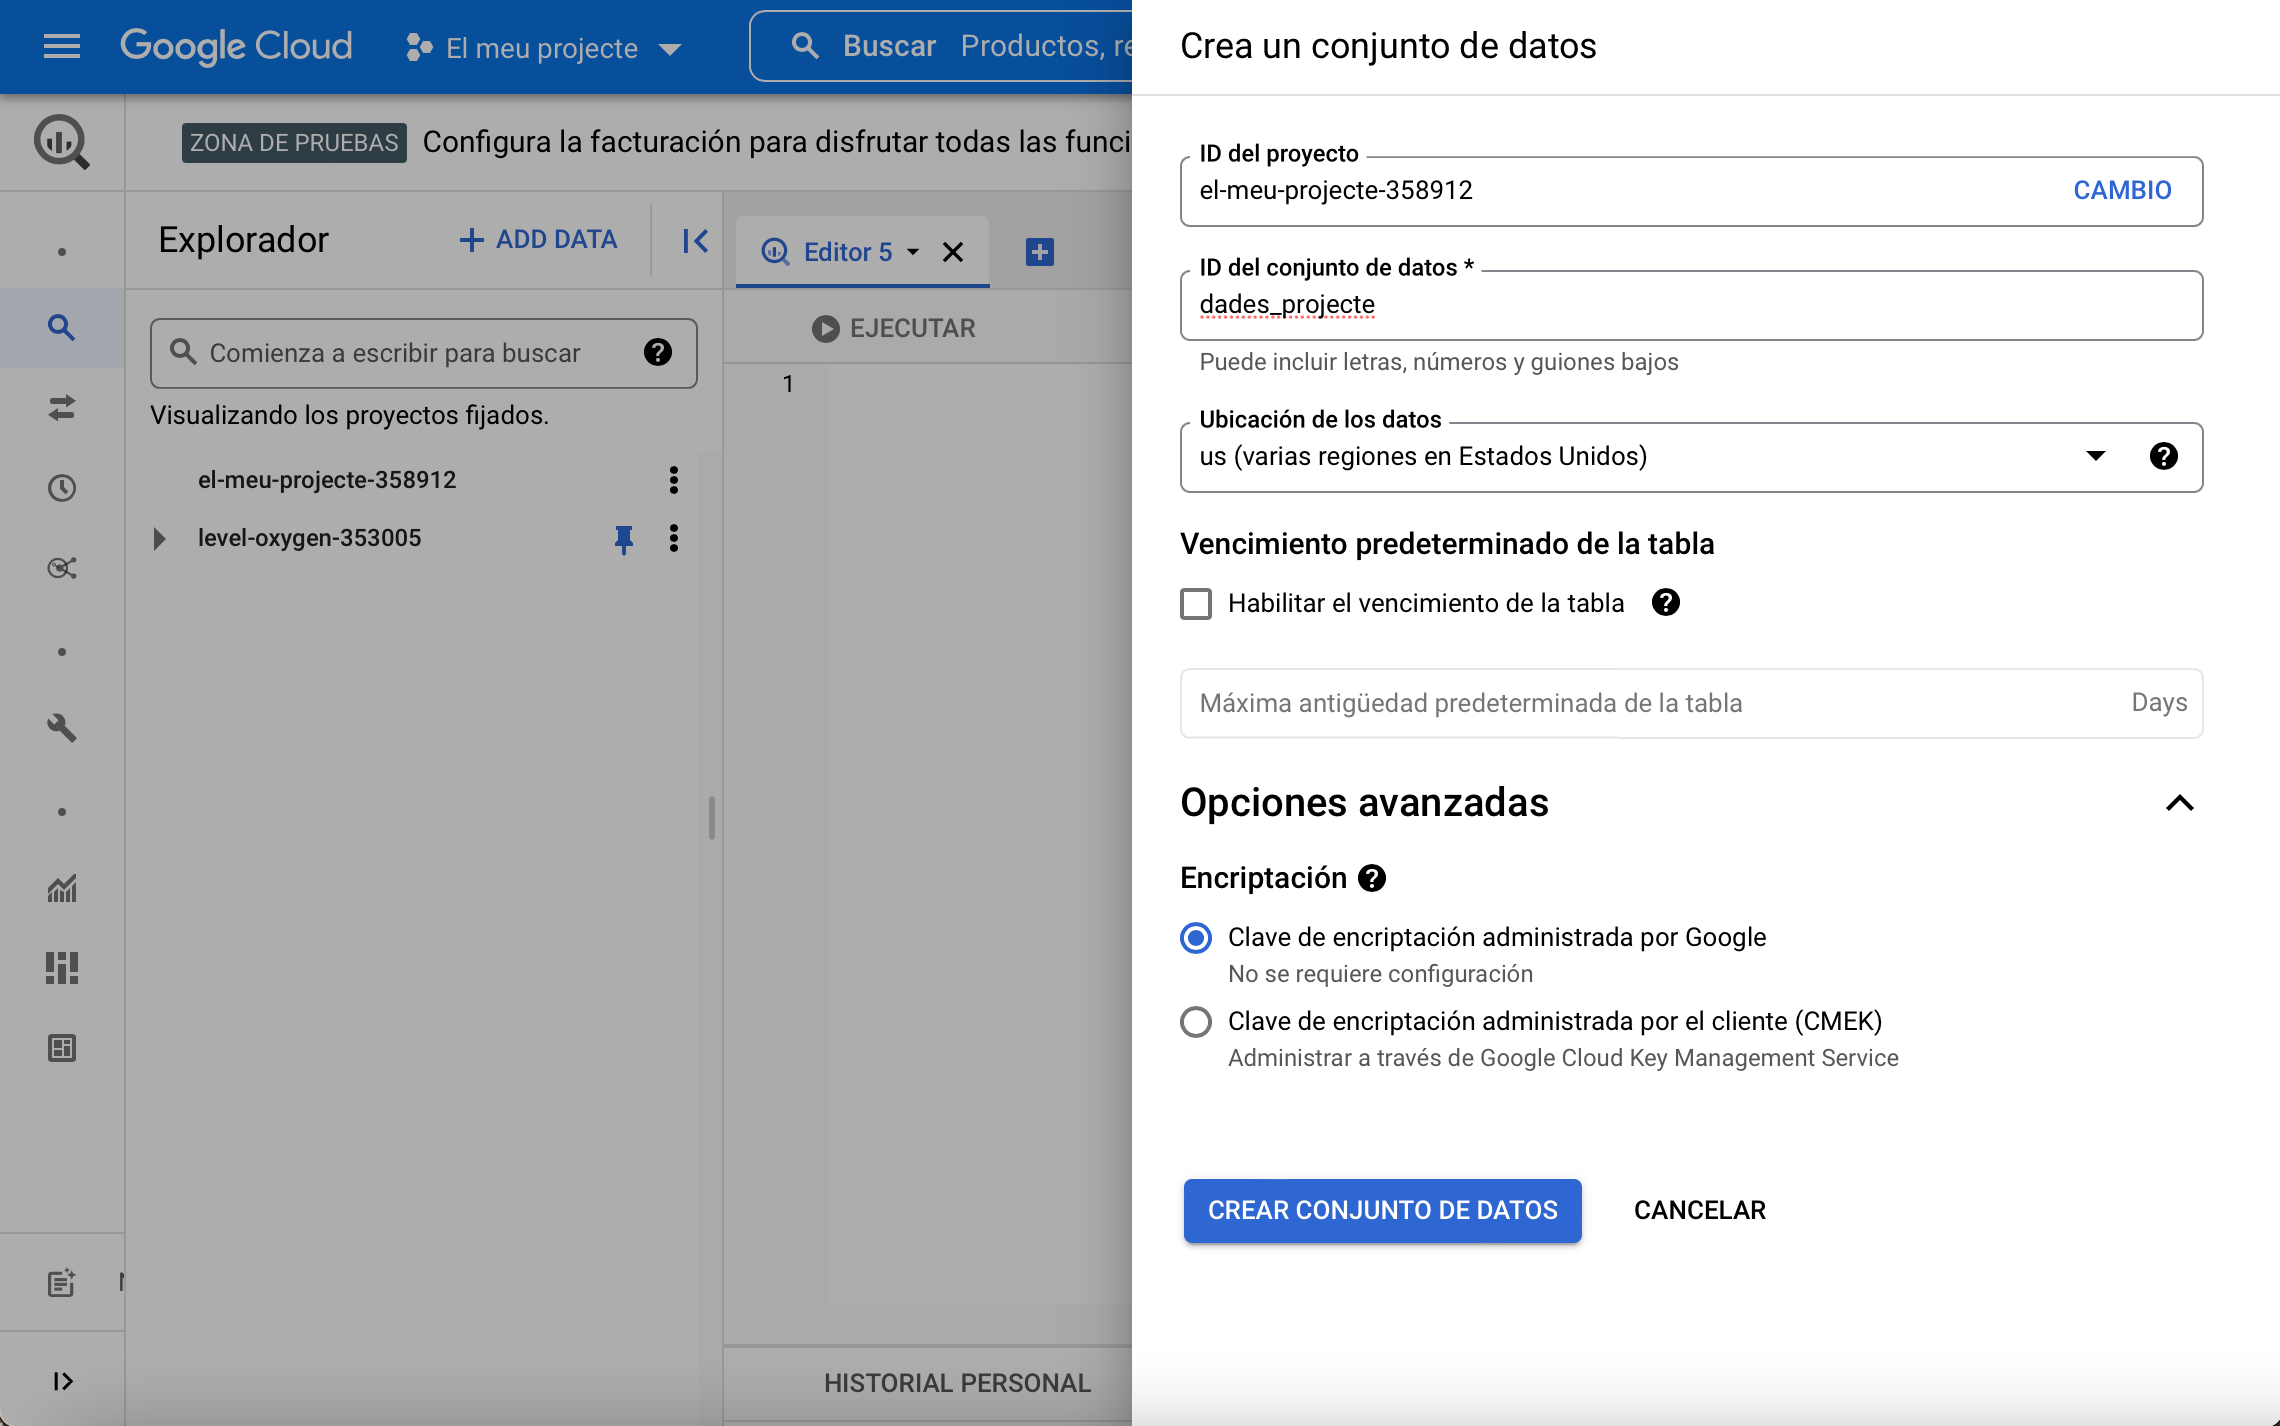
\includegraphics[width=7cm]{bq5}
\end{center}

\subsection{Definició d'una taula de BigQuery des de la interfície d'usuari}

\subsection{Consultar una taula de BigQuery senzilla}

\subsection{Càrrega de dades per crear una taula de BigQuery}

\subsection{Consulta de dades i visualització d'estadístiques de consultes}

\subsection{Creació d'una taula a partir d'un resultat de consulta}

\subsection{Creació d'una consulta a partir d'un filtre}

\newpage

\section{Execució de consultes i visualització de resultats}

\subsection{Conjunts de dades públics a BigQuery}

\subsection{Configuració i ús de memòria cau de BigQuery}

\subsection{Taules externes de BigQuery}

\subsection{Integració de BigQuery amb Data Studio}

\newpage


\end{document}